\documentclass[10pt,twocolumn,letterpaper]{article}

\usepackage{wacv}
\usepackage{times}
\usepackage{epsfig}
\usepackage{graphicx}
\usepackage{amsmath}
\usepackage{amssymb}

% Include other packages here, before hyperref.

% If you comment hyperref and then uncomment it, you should delete
% egpaper.aux before re-running latex.  (Or just hit 'q' on the first latex
% run, let it finish, and you should be clear).
%\usepackage[pagebackref=true,breaklinks=true,letterpaper=true,colorlinks,bookmarks=false]{hyperref}

%\wacvfinalcopy % *** Uncomment this line for the final submission

\def\wacvPaperID{****} % *** Enter the wacv Paper ID here
\def\httilde{\mbox{\tt\raisebox{-.5ex}{\symbol{126}}}}

% Pages are numbered in submission mode, and unnumbered in camera-ready
\ifwacvfinal\pagestyle{empty}\fi
\setcounter{page}{1}
\begin{document}

%%%%%%%%% TITLE
\title{Size to Depth: A New Perspective for Single Image Estination}

% Authors at the same institution
%\author{First Author \hspace{2cm} Second Author \\
%Institution1\\
%{\tt\small firstauthor@i1.org}
%}
% Authors at different institutions
\author{First Author \\
Institution1\\
{\tt\small firstauthor@i1.org}
\and
Second Author \\
Institution2\\
{\tt\small secondauthor@i2.org}
}

\maketitle
\ifwacvfinal\thispagestyle{empty}\fi

%%%%%%%%% ABSTRACT
\begin{abstract}
   %In this paper, we propose a new method for single monocular image depth estimation through human interactions exploiting size information labeled by human instead of traditional geometric or depth information. We divide the image to be processed into equally sized patches, and then label real-world size for the dominant component in each patch manually, or automatically through deep convolutional neural network which is a faster alternative for manual labeling. With size information for each patch, we design an algorithm to generate a coarse depth map. At last we make refinements on the depth map by applying conditional random field. Experimental evaluation shows feasibility and superiority of our method.
We consider the problem of single monocular image depth estimation. It is a notoriously challenging problem due to its ill-posedness nature. Previous efforts can be roughly classified into two families: learning-based method and interactive method. The former, in which deep convolutional neural network (CNN) is adopted frequently, leads to considerable results on specific dataset, but perform poorly on images outside the dataset, which shows its lack of extensiveness. Besides, plenty of data are needed to train the model. The latter requires human annotation of depth which, however, is easily to have large errors.

To overcome these problems, we propose a new perspective for single monocular image depth estimation problem: size to depth. Most previous interactive methods try to obtain depth labels directly from human. Different from these methods, our method receives object size labels from human as prior. Depth can be inferred through simple geometric relationships given size labels. Then we design a conditional random field (CRF) model to propagate depth information and finally generate the whole depth map. We experimentally demonstrate that our method outperforms traditional depth-labeling methods.
\end{abstract}

%%%%%%%%% BODY TEXT
\section{Introduction}

%Single image depth estimation is an essential problem in computer vision which has found various applications in tasks like generating depth for a dataset without depth label and estimate depth for imaginary images such as cartoon. As an important component of understanding geometric relations within a scene, it also serves as a basis for plenty of advanced problems. Single image depth estimation is a quite challenging task for its ill-posedness due to the inherent ambiguity of single images. Learning-based methods are recently proved to be an effective solution, but with two major shortcomings. Firstly, state-of-art methods based on deep neural network require plenty of training data, while RGB-D datasets generated by devices like Kinect and Lidar are limited in both number of images and type of scene. Popular RGB-D datasets such as NYU Depth \cite{silberman11indoor, Silberman:ECCV12} and SUN RGB-D \cite{SUN} typically contain images of indoor scenes less than or on the order of million. Secondly, for unseen images that are not of the same type with training data (\eg, using a neural network trained by indoor scenes to predict depth for images of outdoor scenes), learning-based methods may perform information or depth for several pixels or label relative relationships of depth for some pairs or groups of pixels. Our method belongs to the latter family, which requires only real-world size label from human, instead of depth or geometric information in traditional algorithms. Because labeling size is an much easier task for human compared to labeling depth or geometric information, our method takes advantage. What's more, we try to use machine to label size, which makes labeling extremely efficient.

Single image depth estimation is a fundamental problem which has found wide applications in computer vision. It is a challenging problem for its ill-posedness due to the inherent ambiguity of single monocular image. Some previous works \cite{} try to introduce human prior by exploiting human ability of estimating depth. With manually labeled depth information for several intentionally-selected pixels or patches, the whole depth map is generated by propagating using particular algorithm. Since this method is prone to propagate errors, depth labels in relatively high precision are required. However, human do not perform satisfactorily in depth labeling (as we will show in the experiment section), which becomes a bottleneck for the method.

Different from the previous work, we propose to exploit human ability of estimating object size, which is a new perspective to solve the problem. Compared to previous works where human directly label depth, our method takes significant advantages. Firstly, our experiment shows a relative error of roughly 8\% when human label object size and about 30\% when human label depth, and size-labeling method outperforms depth-labeling method in all the metrics in our setting. Secondly, in practice human label size much faster than labeling depth as size is a quite trivial measure in daily life.

To sum up, we highlight the main contributions of this work as follows:
\begin{itemize}
\item We propose a new perspective for single monocular image depth estimation problem: from size to depth. Given manually labeled size for some objects in image, we are able to infer relative depth through simple geometric relationships. 
\item We design a special conditional random field (CRF) model to apply depth propagation and finally generate the whole depth map.
\item We demonstrate the superiorities of our method compared to the traditional depth-labeling method.
\end{itemize}

%In this paper, we propose a new method which estimates depth also by user interaction requiring size-related information from user instead of geometric or depth-related information. In our method, we firstly divide the image to be processed into small patches, and label approximate size for each patch. Then we... As human are able to describe the size of an object easier than to estimate the depth of an object in an image though daily experience, our method achieves good results and allows users to get rid of 

%-------------------------------------------------------------------------
\section{Related works}

Increasing number of methods are trying to estimate depth for single monocular image, which can be roughly classified into two families: learning-based method and interactive method.

Some traditional learning-based methods formulate depth estimation as a markov random field (MRF) learning problem. Saxena \etal \cite{NIPS2005_2921} use linear regression and MRF to predict depth from a set of image feature. Liu \etal \cite{Liu_2014_CVPR} propose a discrete-continuous conditional random field (CRF) model to take relations between adjacent superpixels into consideration. Realizing the strong correlation between depth estimation and semantic segmentation, Liu \etal \cite{Liu+al:CVPR10} make use of predicted semantic labels to guide 3D reconstruction by enforcing depth related to class and geometry prior.

Most of recent learning-based approaches rely on the application of deep learning, among which deep convolutional neural network (CNN) is used most commonly. Eigen \etal \cite{DBLP:journals/corr/EigenPF14} design a global coarse-scale deep CNN to regress a rough depth map directly from an input image. They then train a local fine-scale network to make local refinements. Liu \etal \cite{Liu_2015_CVPR} propose a deep convolutional neural field model for depth estimation by exploring CNN and  CRF. They jointly learn the unary and pairwise potentials of CRF in a unified deep CNN framework. Like in traditional learning-based method, Wang \etal \cite{Wang_2015_CVPR} use a deep CNN to jointly predict a global layout composed of pixel-wise depth values as well as semantic labels, and improved performance by allowing interactions between depth and semantic information. 

Compared to our method, learning-based methods require plenty of ground truth data and are not able to generalize to unseen images outside the dataset. Some of the methods \cite{Liu+al:CVPR10, Wang_2015_CVPR} need result of segmentation algorithm.

Human interactive methods exploit human ability to interpret 2D images, using human annotation. Some previous works make use of geometric elements (lines or plains) in images to predict depth. Criminisi \etal \cite{Criminisi2000} describe a way to compute 3D affine measurements given human inputs providing geometric information determined from the image. Later works \cite{Lee2009GeometricRF} by Lee \etal try to generate plausible interpretations of a scene from a collection of line segments automatically extracted from a single indoor image. These methods are limited for requiring a large amount of straight lines or plains in the image to provide enough evidences for 3D structure inference. Lopez \etal \cite{ceig.20141109} formulate the problem as an optimization process by assuming that image regions with low gradients will have similar depth values. In their method, depth values are propagated between pixels with small image gradients under a number of human-defined constraints. Our method, In contrast, requires only size information, which is more trivial for human to label than geometric or depth information. We will show this in the following sections.

\section{Our method}
// Notations, conventions

\subsection{Overview}
%Our goal is to estimate pixelwise depth for single image of general cases. The ability of inferring depth in human brain depends extensively on its knowledge of objects and their spatial relations. Inference of depth should be made on the basis of knowledge of 3d shape of real-world objects as well as understanding of 3d space. However, learning-based methods performing depth estimation is basically built on 2d images. Learning-based methods built on such data are forced to work out depth which requires 3d understanding given training information of lower dimension, introducing much ill-posedness to the problem.  Besides, RGBD datasets generated by devices like Kinect and Lidar is limited in both type of scene and number of images. Popular RGBD datasets such as NYU Depth or SUN RGBD typically contain images of indoor scenes less than or on the order of million. Such low dimension, biased and inadequate data is not sufficient for applying an NN-based method. Another point is, a model haven't been developed that has level of understanding of 3d space and spatial relation the task requires. We are still working on asking questions like counting number of objects which is a much much simpler problem than reasoning spatial relation in 3d space. Neither gain knowledge of 3d object shape nor inferring spatial relation is solved as a single problem, and learning-based methods are asking neural networks to do both for depth estimation. Thus, learning-based methods, at least in this time, is not sufficient to handle this task on its own.
Our goal is to estimate pixelwise depth for single image of general cases. We develop an algorithm that takes advantage of human annotation to estimate depth. Note that, directly labeling depth of pixel in numeric value is impractical for humans. Senses of human are involved to be sensitive to comparing relative depth but not estimating raw value of depth. One can readily distinguish the nearer object between two, but struggles to name that distance to an object is 10m, 12m or 15m. The basic equation in computer vision
\begin{equation}
\text{depth} \propto \text{focal\ length} * \frac{\text{real-world\ size}} {\text{size\ in\ photo}}
\end{equation}
implies that depth of object is proportional to its real-world size given focal length and its size in photo is fixed, which is satisfied in our problem setting. And labeling real-world size of objects is a much better formulation of annotation since size of objects is common knowledge for human.
\par
In order to simplify the labeling process while get global layout of depth by annotation, we propose a patch-to-size way of annotation. In this formulation, image is divided into grids of equally sized patches. And human are asked to label real-world size of dominant component in each patch. To involve both local and global horizon, this is done several times for coarse-to-fine patch division of image.
\par
After patch-to-size step, we obtain size for each patch (which is equivalent to depth). But the result is rather coarse with rigid boundary. Another depth refinement step is introduced to smooth depth gaps and interpolate between pixels under the constraint of depth annotation. 
\par
The depth refinement step is formulated as an energy function optimization problem in conditional random field (CRF). Mathematically, let $\mathbf{x}$ be the RGB-D image, $\mathbf{y}$ be the corresponding depth, $\mathbf{\theta}$ be the model parameter (if any, \eg parameters of patch-to-size CNN), we model the conditional probability distribution of RGB-D data with
\begin{equation}
\text{Pr}(\mathbf{y}|\mathbf{x}, \mathbf{\theta}) = \frac{1}{Z(\mathbf{x}|\mathbf{\theta})}\text{exp}(-E(x, y|\mathbf{\theta}))
\end{equation}
where $E(\mathbf{x}, \mathbf{y}|\mathbf{\theta})$ is the energy function and $Z(\mathbf{x}|\mathbf{\theta})$ is a normalization term given by
\begin{equation}
Z(\mathbf{x}) = \int_y\text{exp}(-E(\mathbf{x}, \mathbf{y})) dy.
\end{equation}
Model parameter $\theta^*$ that best fits the training data is found by maximum likelihood estimation with regularization
\begin{equation}
\theta^* = \text{argmax}_{\theta} \log \text{Pr}(\mathbf{y}|\mathbf{x}, \mathbf{\theta}) + \text{reg}(\mathbf{\theta}).
\end{equation}
And maximum a posteriori (MAP) solution $\mathbf{y}^*$ gives the depth $\mathbf{y}$ of maximum probability for observed image $\mathbf{x}$ which is the best estimation of depth
\begin{equation}
\mathbf{y^*} = \text{argmax}_{\mathbf{y}} \log \text{Pr}(\mathbf{y}|\mathbf{x}, \mathbf{\theta}).
\end{equation}
\par
In the following, we will give a detailed discussion about components of our algorithm.
\subsection{Annotation formulation}
As discussed, knowledge of object shape and spatial relation is fundamental for depth estimation. Realizing the difficulty to model them by learning, we introduce human knowledge to ease the urge. And we must decide whose size to label. Having the annotator draw the contour of labelled object would be too complex and time-consuming. We come up with the patch dividing idea to avoid this problem. In our patch-to-size formulation, specification of labelled object is substituted by a flexible concept of dominant component. Patch-to-size makes the general assumption that depth of dominant component in the patch is representative of the entire patch(this does not mean we will assign same depth for every pixel in the patch, refer to Section 3.4). The assumption is definitely inapplicable in some cases such as images depicting a person in the background of sky. But it can be fixed by introducing CRF loss terms as shown in section 3.4.
\subsection{Faster alternative for manual labeling}
Although patch-to-size greatly reduces annotation effort, one still have to label up to 10 by 10 patches which takes 3-5 minutes. We make the attempt to speedup this process by learning to label size by CNNs. Different CNNs are trained for each granularity of patch division. [Description of CNN architecture, need more experiment]
\subsection{Conditional random field}
As is typically formulated, energy function of CRF consists of unary and binary potential terms.
\begin{align}
E(\mathbf{x}, \mathbf{y}) &= \sum_{p \in P}E_{unary}(y_{p}, \mathbf{x}) \\ &\quad + \lambda \sum_{x, y \in A} \frac{1}{2} E_{binary}(y_x, y_y, \mathbf{x})
\end{align}
where $P$ is the set of pixels in the image, $A$ is set of adjacent pair of pixels. $E_{unary}\text{ and }E_{binary}$ are relatively unary and binary loss terms.
\par
The unary term is given by
\begin{align}
E_{unary}(y_{p}, \mathbf{x}) &= (y_p - \sum_i{w_i d_i})^2
\\ &=(y_p-w^T\mathbf{d})^2
\end{align}
where $d_i$ is the depth annotation. This term basically requires the depth of image to match with depth of its belonging patches.
\par
The binary term is given by
\begin{equation}
E_{binary}(y_x, y_y, \mathbf{x}) = \text{sim}(x, y) (y_x-y_y)^2
\end{equation}

where $\text{sim}(x, y)$ is a similarity function of pixel. This term penalizes gap of depth between neighboring pixels which encourages local continuity of the depth field.
Similarity between pixels can be represented by image gradient
\begin{equation}
\text{sim}(x, y) = |I_x-I_y|
\end{equation}
where $I$ denotes image intensity.
\subsection{MAP in CRF}
In the case of manual annotation, depth $d_i$ is predefined by user, enabling us to pre-process the $w^T\mathbf{d}$ term to be a single variable $d_p$ for every pixel. And if we measure similarity by image gradient, energy function can be written as
\begin{equation}
E(\mathbf{x}, \mathbf{y}) = \sum_{p \in P} (y_p-d_p)^2 + \lambda \sum_{x, y \in A}(I_x-I_y)(y_x-y_y)^2.
\end{equation}
Optimization of $E$ can be performed by taking gradient w.r.t $\mathbf{y}$ and doing gradient descent. Rewrite energy function $E$ as a function of $\mathbf{y}$:
\begin{align}
E &= \mathbf{y}^T (\ (\ 1+\sum_{y, (x, y)\in A}|I_x-I_y|\ )I+W\ )\mathbf{y}-2\mathbf{y}^Td+d^Td 
\\ &= \mathbf{y}^T W'\mathbf{y}-2\mathbf{y}^Td+d^Td 
\end{align}
where I is the identity matrix, d is the vector of $d_p$, $W_{ij} = |I_x-I_y| $ and 
\begin{equation}
W' = 1+\sum_{y, (x, y)\in A}|I_x-I_y|.
\end{equation}
Normalization term $Z$ can be analytically integrated:
\begin{align}
Z(\mathbf{x}) &= \int_y \text{exp}(-E(\mathbf{x}, \mathbf{y})) dy
\\ &= \frac{\pi ^{\frac{n}{2}}}{|W'|^{\frac{1}{2}}}\text{exp}(d^TW'^{-1}d-d^Td).
\end{align}
and the log-likelihood of posterior is given by
\begin{align}
\log \text{Pr}(\mathbf{y}|\mathbf{x}) = \frac{n}{2}\log \pi - \frac{1}{2}|W'|+d^TW'^{-1}d-d^Td
\end{align}
With l2-loss, the objective of CRF can be written as
\begin{equation}
\min \sum \log \text{Pr}(\mathbf{y}| \mathbf{x})
\end{equation}
The optimization problem is efficiently solved by gradient descent.[More detailed derivation of gradient]
\subsection{Maximum likelihood estimation in CRF}
Our CRF also fit in parameterized learning scheme. Parameters might come from the patch-to-size CNN to speed up patch-to-size. In that case, 
\begin{equation}
E_{unary} = (y_p - w^T\mathbf{d}(\mathbf{\theta}))^2
\end{equation}
and the final gradient w.r.t $\mathbf{\theta}$ is given by
\begin{align}
\frac{\partial E_{unary}}{\partial \mathbf{\theta}} &= \frac{\partial E_{unary}}{\partial \mathbf{d}}\frac{\partial \mathbf{d}}{\partial \mathbf{\theta}}
\\ & = \sum \mathbf{y} \text{grad}(\mathbf{\theta})
\end{align}
where $\text{grad}(\mathbf{\theta})$ is calculated by back propagation in CNN.
\par
Another possible parameterization is by applying CNN as distance metric. Note that inferring depth on pixelwise scale in CRF is computationally extensive. Thus we can infer in larger scale patches in CRF while generate finer-grain depth map by upsample. Designing a reasonable mathematical representation of distance metric between patches is nontrivial. Thus we introduce CNN to perform a projection from high-dimension image space to low-dimension distance space where euclidean distance of feature vector is representative of distance between patches. In this setting, 
\begin{align}
E_{binary}(y_x, y_y, \mathbf{x}) &= \text{sim}(x, y, \mathbf{\theta}) (y_x-y_y)^2
\\ &= (f(x, \mathbf{\theta})-f(y, \mathbf{\theta}))^2(y_x-y_y)^2
\end{align}
where $f(\mathbf{x}, \mathbf{\theta})$ is the transform function defined by the CNN. The final gradient w.r.t $\mathbf{\theta}$ is given by
\begin{align}
\frac{\partial E_{binary}}{\partial \mathbf{\theta}} &=\sum 2(f(x, \mathbf{\theta})-f(y, \mathbf{\theta}))(\text{grad}(\mathbf{x}, \theta)-\text{grad}(\mathbf{y}, \theta))
\\& (y_x-y_y)^2
\end{align}
The projection CNN can be optimized by performing back propagation.

\section{Experiment}
\subsection{}
We test images from NYU Depth V2 dataset and use our algorithm to generate depth map for it. Processing a standard image with size $480 \times 640$ takes tens of seconds. Some of the results are shown in Figure .

\begin{figure*}
\begin{center}
\fbox{\rule{0pt}{0in} \rule{0\linewidth}{0pt}
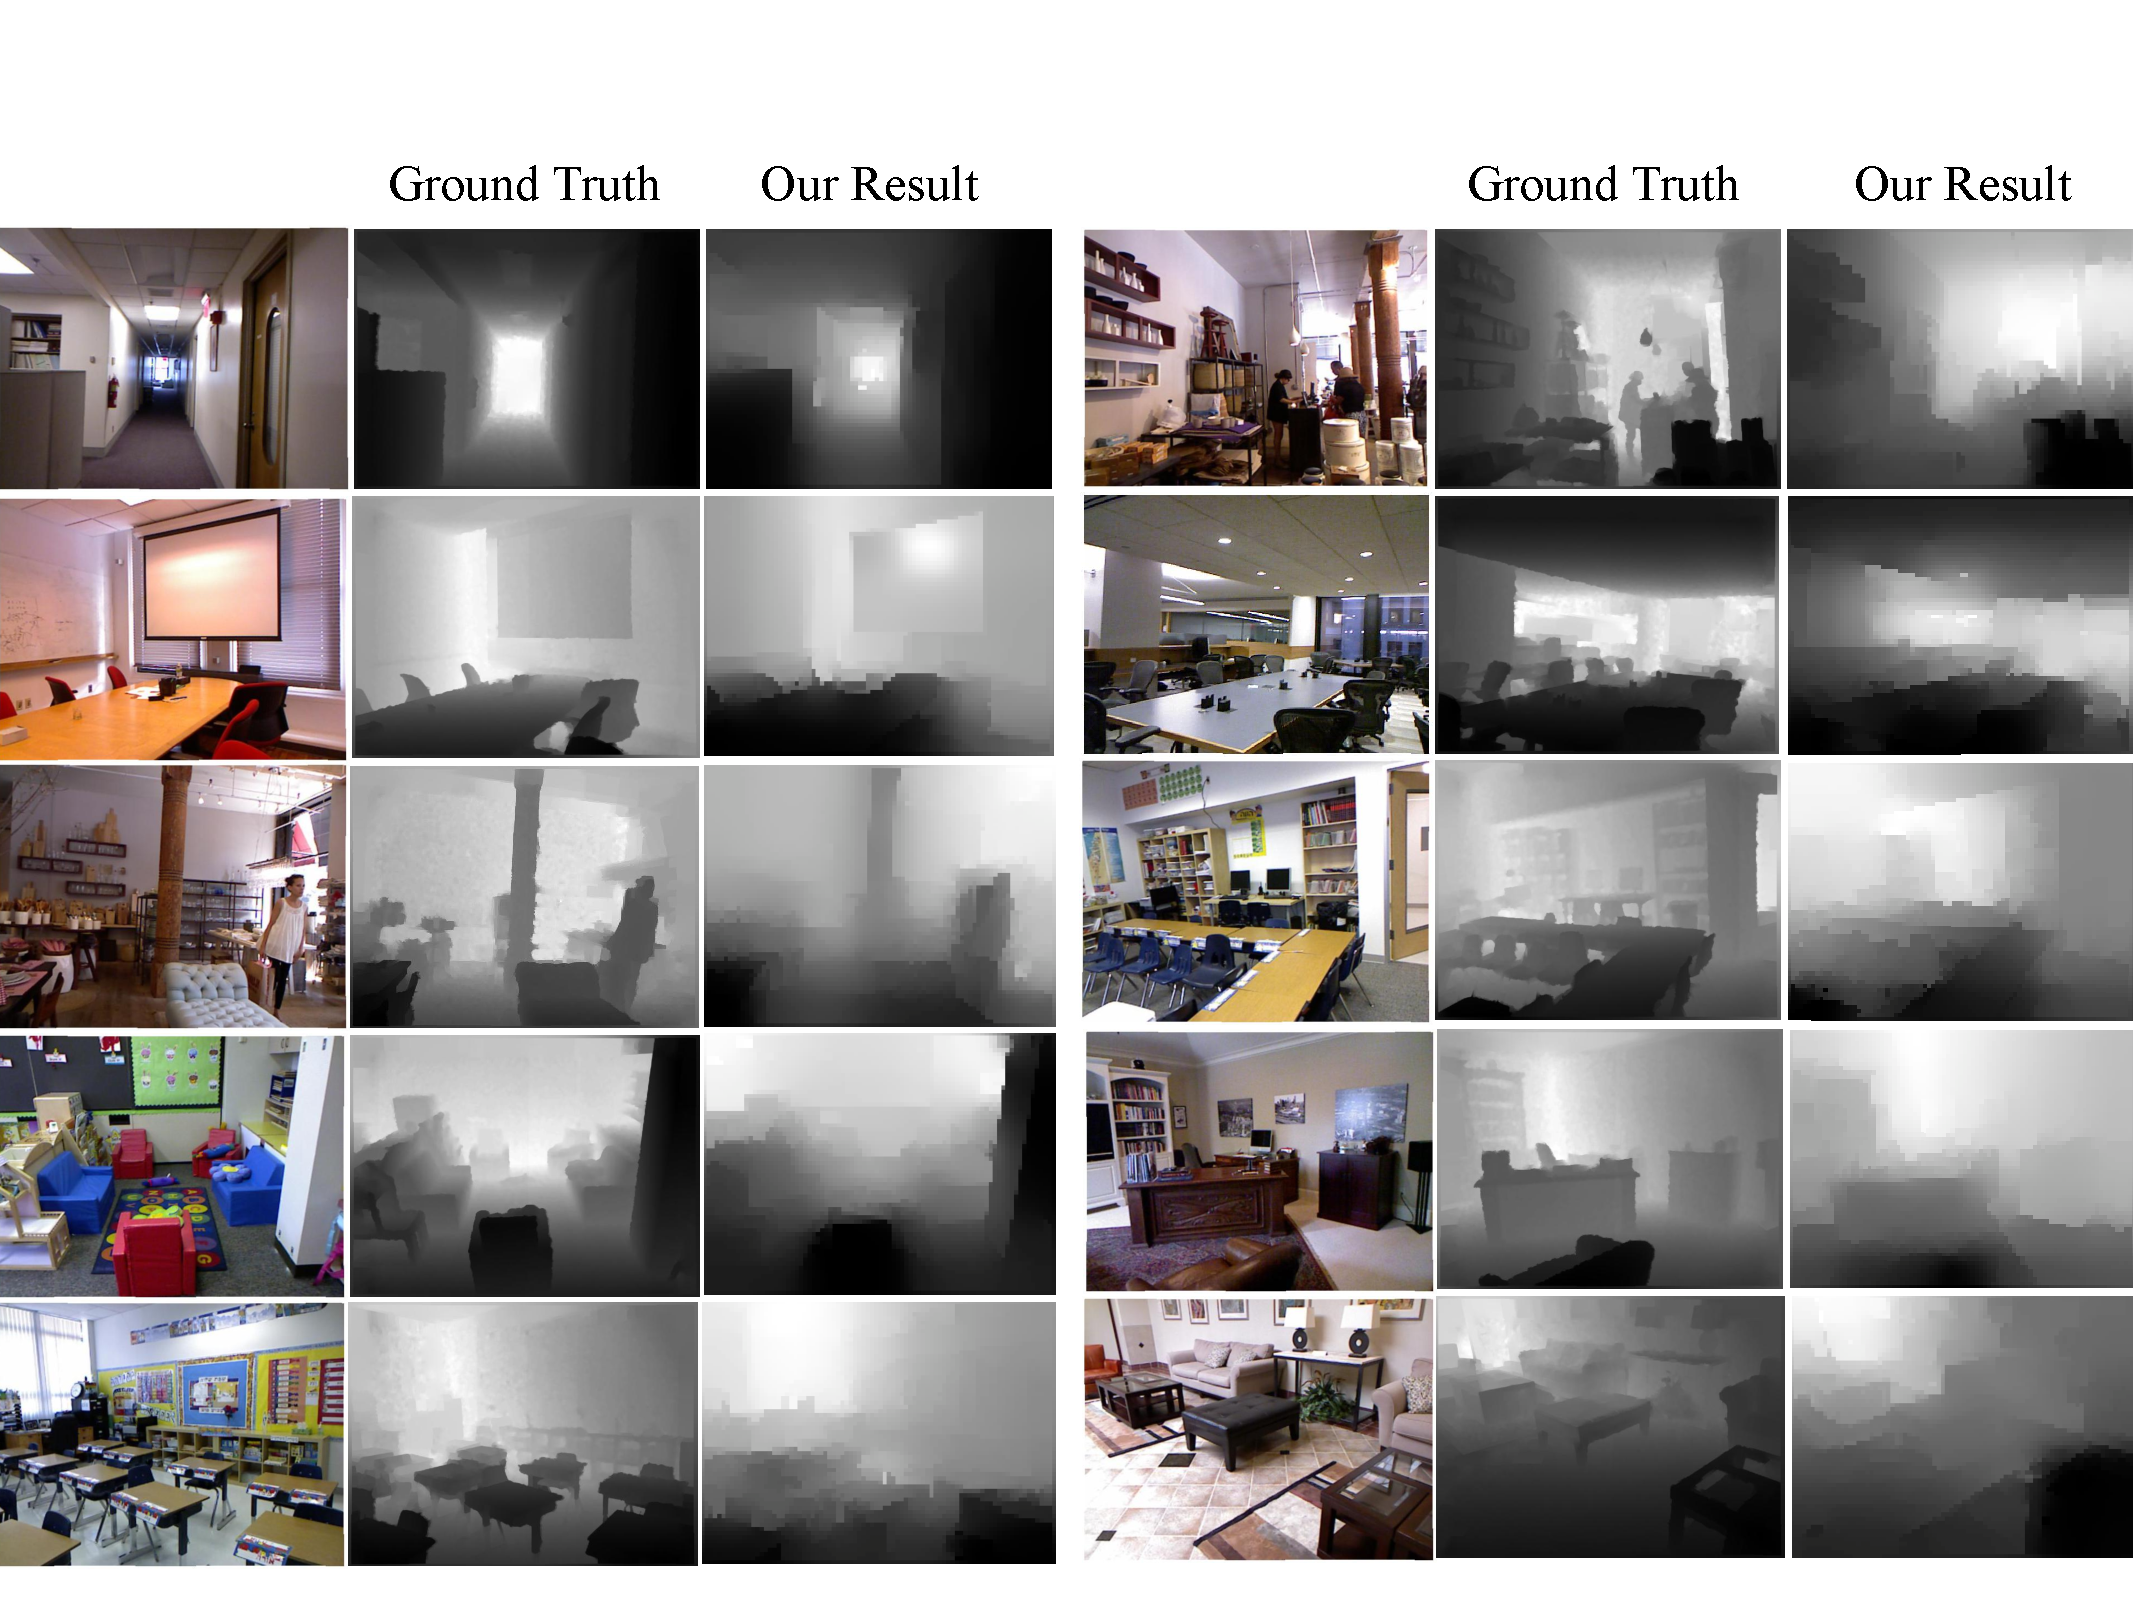
\includegraphics[width=16cm]{demos.pdf}}
\end{center}
   \caption{Example of a short caption, which should be centered.}
\label{fig:short}
\end{figure*}


{\small
\bibliographystyle{ieee}
\bibliography{egbib}
}


\end{document}
